\documentclass[12pt,twoside]{reedthesis}
\usepackage{graphicx,latexsym} 
\usepackage{amssymb,amsthm,amsmath}
\usepackage{longtable,booktabs,setspace} 
\usepackage[hyphens]{url}
\usepackage{rotating}
\usepackage{natbib}
\usepackage[margin=1in]{geometry}
\usepackage{clrscode3e}
\usepackage{mathtools}
\usepackage{tikz}
\usepackage{float}
\usetikzlibrary{positioning,arrows}
\usepackage{setspace}
\usepackage{mathpazo}
\doublespacing
%\usepackage{tikz-berge}
%\usepackage{algorithm}
%\usepackage[noend]{algpseudocode}

 
\newcommand{\N}{\mathbb{N}}
\newcommand{\Z}{\mathbb{Z}}
\newcommand{\R}{\mathbb{R}}
\renewcommand{\'}{^{'}}
\renewcommand{\gets}{:=}
 
\newenvironment{theorem}[2][Theorem]{\begin{trivlist}
\item[\hskip \labelsep {\bfseries #1}\hskip \labelsep {\bfseries #2.}]}{\end{trivlist}}
\newenvironment{lemma}[2][Lemma]{\begin{trivlist}
\item[\hskip \labelsep {\bfseries #1}\hskip \labelsep {\bfseries #2.}]}{\end{trivlist}}
\newenvironment{definition}[2][Definition]{\begin{trivlist}
\item[\hskip \labelsep {\bfseries #1}\hskip \labelsep {\bfseries #2.}]}{\end{trivlist}}
\newenvironment{problem}[2][Problem]{\begin{trivlist}
\item[\hskip \labelsep {\bfseries #1}\hskip \labelsep {\bfseries #2.}]}{\end{trivlist}}
\newenvironment{question}[2][Question]{\begin{trivlist}
\item[\hskip \labelsep {\bfseries #1}\hskip \labelsep {\bfseries #2.}]}{\end{trivlist}}


% Comment out the natbib line above and uncomment the following two lines to use the new 
% biblatex-chicago style, for Chicago A. Also make some changes at the end where the 
% bibliography is included. 
%\usepackage{biblatex-chicago}
%\bibliography{thesis}

% \usepackage{times} % other fonts are available like times, bookman, charter, palatino

\title{Thesis}
\author{Zachary Campbell}
\date{May 2018}
\division{Mathematics and Natural Sciences}
\advisor{Jim Fix}
\department{Mathematics}
\setlength{\parskip}{0pt}

%% The fun begins:
\begin{document}

  \maketitle
  \frontmatter % this stuff will be roman-numbered
  \pagestyle{empty} % this removes page numbers from the frontmatter

\chapter*{Acknowledgements}

\tableofcontents

\mainmatter % here the regular arabic numbering starts
\pagestyle{fancyplain} % turns page numbering back on
%The \introduction command is provided as a convenience.
%if you want special chapter formatting, you'll probably want to avoid using it altogether
\chapter*{Introduction}
         \addcontentsline{toc}{chapter}{Introduction}
	\chaptermark{Introduction}
	\markboth{Introduction}{Introduction}
	% The three lines above are to make sure that the headers are right, that the intro gets included in the table of contents, and that it doesn't get numbered 1 so that chapter one is 1.
	
\chapter{Bipartite graphs and matchings}

	In this chapter we review bipartite graphs and matchings, and discuss their relevance to this 
	thesis. We will also begin our discussion of linear programming, in a casual way, to give the 
	reader a taste for what is coming.
\begin{section}{Bipartite graphs and matchings}

	Throughout this thesis we will be interested in a specific subclass of graphs known as 
	bipartite graphs. Unless otherwise noted, our algorithms will assume a bipartite structure.

	\begin{definition}
		A \emph{bipartite graph} is a graph whose vertices can be partitioned into two 
		sets $U$ and $V$ such that all edges connect a vertex $u\in U$ to a vertex $v\in V$.
		We will denote this graph $G = (U,V,E)$, where $E$ is the edge set $(U\times V)$.
	\end{definition}	
	\begin{figure}[h]
		\centering
	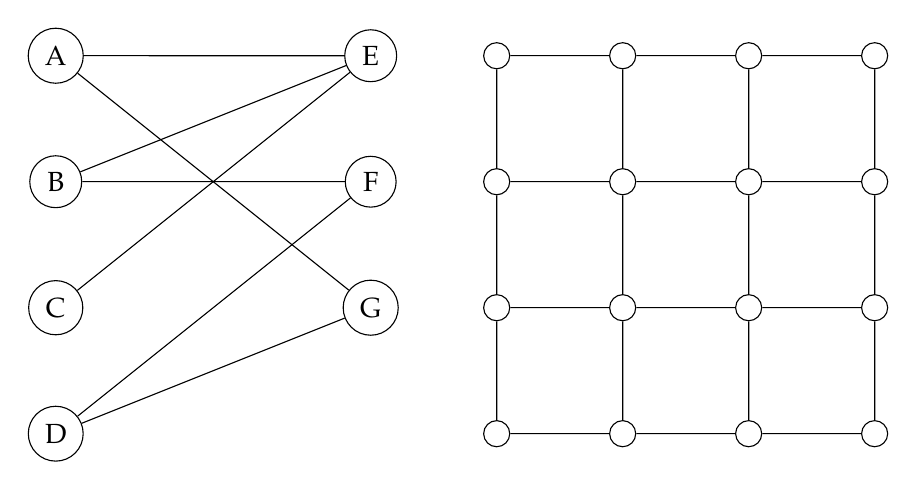
\begin{tikzpicture}[scale=.8,auto=left,every node/.style={circle,draw=black}]
		%left nodes
		\node (n1) at (1,10) {A};
		\node (n2) at (1,8) {B};
		\node (n3) at (1,6) {C};
		\node (n4) at (1,4) {D};

		%right nodes
		\node (n5) at (6,10) {E};
		\node (n6) at (6, 8) {F};
		\node (n7) at (6, 6) {G};
		
		%edges
		\draw (n1) -- (n5);
		\draw (n1) -- (n7);
		\draw (n2) -- (n5);
		\draw (n2) -- (n6);
		\draw (n3) -- (n5);
		\draw (n4) -- (n6);
		\draw (n4) -- (n7);

		%left nodes
		\node (n1) at (8,10) {};
		\node (n2) at (8,8) {};
		\node (n3) at (8,6) {};
		\node (n4) at (8,4) {};

		%center left nodes
		\node (n5) at (10,10) {};
		\node (n6) at (10,8) {};
		\node (n7) at (10,6) {};
		\node (n8) at (10,4) {};

		%center right nodes
		\node (n9) at (12,10) {};
		\node (n10) at (12,8) {};
		\node (n11) at (12,6) {};
		\node (n12) at (12,4) {};

		%right nodes
		\node (n13) at (14,10) {};
		\node (n14) at (14,8) {};
		\node (n15) at (14,6) {};
		\node (n16) at (14,4) {};

		%edges
		\draw (n1) -- (n2);
		\draw (n1) -- (n5);
		\draw (n2) -- (n3);
		\draw (n2) -- (n6);
		\draw (n3) -- (n4);
		\draw (n3) -- (n7);
		\draw (n4) -- (n8);
		\draw (n5) -- (n6);
		\draw (n5) -- (n9);
		\draw (n6) -- (n7);
		\draw (n6) -- (n10);
		\draw (n7) -- (n8);
		\draw (n7) -- (n11);
		\draw (n8) -- (n12);
		\draw (n9) -- (n10);
		\draw (n9) -- (n13);
		\draw (n10) -- (n11);
		\draw (n10) -- (n14);
		\draw (n11) -- (n12);
		\draw (n11) -- (n15);
		\draw (n12) -- (n16);
		\draw (n13) -- (n14);
		\draw (n14) -- (n15);
		\draw (n15) -- (n16);
	\end{tikzpicture}
	\caption{Examples of bipartite graphs}
	\end{figure}
	In Figure 1.1 we have a bipartite graph with vertex partition given by $U = \{A,B,C,D\}$ and 
	$V = \{E,F,G\}$. All edges in this graph are between a node $u\in U$ and a node $v\in V$. The 
	graph on the right is also bipartite. It may take a little more time to convince yourself that 
	you can partition the vertices into disjoint $U$ and $V$ in a way that maintains the 
	bipartite property. Try it!
	Now that we know what we are working with, let's introduce a problem that 
	we'd like to solve on these graphs.  
	\begin{definition}
		Let $G = (U,V,E)$ be a bipartite graph. A subset $M\subset E$ is a \emph{matching} if 
		no two edges in $M$ are incident to the same vertex. We call a matching 
		\emph{perfect} if all vertices are an endpoint of an edge in $M$.
	\end{definition}
	We say that a vertex $w\in U\cup V$ is \emph{matched} with respect to $M$ if it is an endpoint 
	of some edge in $M$. The following figure shows some examples of different matchings on one 
	of the graphs from Figure 1.1, where the bold edges are the edges in the matching.
	\begin{figure}[h]
		\centering
		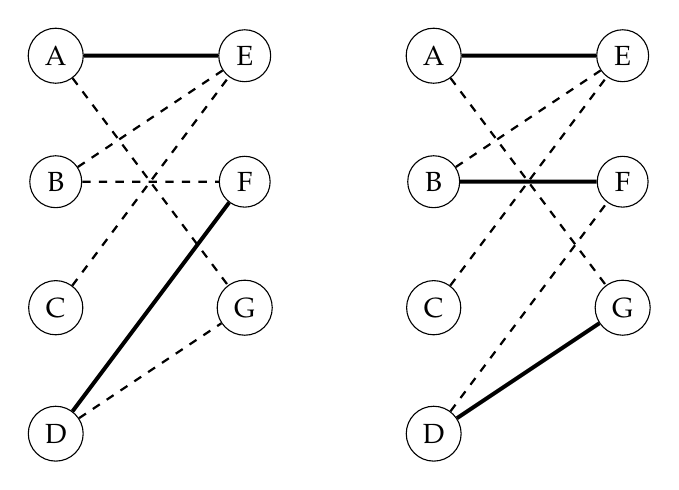
\begin{tikzpicture}[scale=.8,auto=left,every node/.style={circle,draw=black}]
		
		%left nodes
		\node (n1) at (1,10) {A};
		\node (n2) at (1,8) {B};
		\node (n3) at (1,6) {C};
		\node (n4) at (1,4) {D};

		%right nodes
		\node (n5) at (4,10) {E};
		\node (n6) at (4, 8) {F};
		\node (n7) at (4, 6) {G};
		
		%edges
		\draw[line width=0.5mm] (n1) -- (n5);
		\draw[thick,dashed] (n1) -- (n7);
		\draw[thick,dashed] (n2) -- (n5);
		\draw[thick,dashed] (n2) -- (n6);
		\draw[thick,dashed] (n3) -- (n5);
		\draw[line width=0.5mm] (n4) -- (n6);
		\draw[thick,dashed] (n4) -- (n7);

		%left nodes
		\node (m1) at (7,10) {A};
		\node (m2) at (7,8) {B};
		\node (m3) at (7,6) {C};
		\node (m4) at (7,4) {D};

		%right nodes
		\node (m5) at (10,10) {E};
		\node (m6) at (10, 8) {F};
		\node (m7) at (10, 6) {G};
		
		%edges
		\draw[line width=0.5mm] (m1) -- (m5);
		\draw[thick,dashed] (m1) -- (m7);
		\draw[thick,dashed] (m2) -- (m5);
		\draw[line width=0.5mm] (m2) -- (m6);
		\draw[thick,dashed] (m3) -- (m5);
		\draw[thick,dashed] (m4) -- (m6);
		\draw[line width = 0.5mm] (m4) -- (m7);

		\end{tikzpicture}
		\caption{Examples of matchings on a bipartite graph}
	\end{figure}
	There many different valid matchings on the graph in Figure 1.2. Oftentimes, we want to find 
	the largest matching on a graph. This is classically motivated by economic examples, where we 
	have a set of bidders, and a set of goods, and the edges between them denote a bidder $i$'s 
	willingness to pay for good $j$. For a money-hungry auctioneer, the goal here would be to 
	find the ``largest'' matching on the graph, i.e. the one that maximizes profit of the auction. 
	We will discuss this interpretation in more depth later on in the thesis, but it naturally 
	leads to the following definition.
	\begin{definition}
		A \emph{maximal matching} on $G$ is a matching $M$ such that if any other edge 
		not in $M$ is added to $M$, it is no longer a valid matching. Alternatively put, 
		$M$ is maximal if there is no matching $M\'$ such that $M\subset M\'$.
	\end{definition}
	Both matchings in Figure 1.2 are maximal matchings; in each case there are no edges that 
	we can add to $M$ and have that $M$ is still a matching. However, notice that these matchings 
	have different sizes, even though both are maximal on $G$. This leads to the following 
	definition.
	\begin{definition}
		A matching $M$ on a graph $G$ is said to be a \emph{maximum matching} if for all other 
		matchings $M\'$ on $G$, $|M\'| \leq |M|$.
	\end{definition}
	In our example, the matching on the right given by $M = \{(A,E), (B,F), (D,G)\}$ is a 
	maximum matching (convince yourself). In general there may be many unique maximum matchings 
	on a graph.\\
	In this section we are interested in general methods for finding maximum matchings on 
	bipartite graphs. One of the fundamental approaches is to look at certain subgraphs called 
	alternating paths. Before we define what these are, let's look at a motivating example.
	Suppose we have the matching on the left in Figure 1.2. So $M = \{(A,E),(D,F)\}$. Consider 
	the following sequence of vertices in the graph:
	\begin{figure}[h]
		\centering
		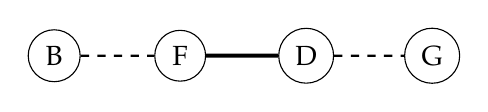
\begin{tikzpicture}[scale=.8,auto=left,every node/.style={circle,draw=black}]

			\node (n1) at (1,10) {B};
			\node (n2) at (3,10) {F};
			\node (n3) at (5,10) {D};
			\node (n4) at (7,10) {G};

			\draw[thick,dashed] (n1) -- (n2); 
			\draw[line width=0.5mm] (n2) -- (n3);
			\draw[thick,dashed] (n3) -- (n4);
		\end{tikzpicture}
	\end{figure}
	Call this sequence $p$. Let's perform an 
	operation that we will denote $M\oplus p$, which operates like XOR: add to $M$ each edge in 
	$p$ that isn't in $M$, and remove from $M$ each edge in $p$ that is in $M$. This gives us 
	the following segment, where $(B,F)$ and $(D,G)$ are now in $M$, but $(D,F)$ is not:
	\begin{figure}[h]
		\centering
		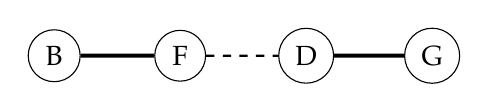
\begin{tikzpicture}[scale=.8,auto=left,every node/.style={circle,draw=black}]

			\node (n1) at (1,10) {B};
			\node (n2) at (3,10) {F};
			\node (n3) at (5,10) {D};
			\node (n4) at (7,10) {G};

			\draw[line width=0.5mm] (n1) -- (n2); 
			\draw[thick,dashed] (n2) -- (n3);
			\draw[line width=0.5mm] (n3) -- (n4);
		\end{tikzpicture}
	\end{figure}
	First, we must check that the new $M$ is still a valid matching; we do this by noticing that 
	$B$ and $G$ were originally unmatched, so it's okay for one of their incident edges to be 
	added. Also, notice that the size of our matching has grown by 1! In fact, this new matching 
	is exactly the matching given by the graph on the right in Figure 1.2. 
	This is a general technique in 
	finding maximum matchings. We want to look for these paths that start and end at unmatched 
	vertices, and whose edges are alternately matched and unmatched. If we can find one of these 
	paths, we will be able to increase the size of matching. We define this formally now.
	\begin{definition}
		Let $G$ be a graph and $M$ some matching on $G$. An \emph{alternating path} is a 
		sequence of vertices and edges that begins with an unmatched vertex, and whose 
		edges alternate between being in $M$ and not in $M$.
	\end{definition}
	\begin{definition}
		An \emph{augmenting path} is an alternating path that starts and ends on unmatched 
		vertices. When we augment $M$ by an augmenting path $p$, we use the notation 
		$M\oplus p$.
	\end{definition}
	This motivates a general method for finding a maximum matching on a bipartite graph: 
	just keep looking for augmenting paths, and augment the current matching by that augmenting 
	path. Of course, we need to prove that this in fact gives us a maximum matching. The following 
	theorem says exactly that.
	\begin{theorem}{(Berge, 1957)}
		A matching $M$ on $G$ is a maximum matching if and only if $G$ contains no augmenting 
		paths with respect to $M$.
	\end{theorem}
	This gives us the following framework for finding maximum matchings in bipartite graphs.
		\begin{codebox}
			\Procname{$\proc{Maximum-matching algorithm} (G)$}
			\li $M \gets \emptyset $
			\li $\While$ $\exists$ an augmenting path $p$
				\Do
			\li		$M \gets M\oplus p$
				\End
			\li $\Return$ $M$
		\end{codebox}
	Note that we have yet to describe the details of this algorithm. Before we do so, we are going 
	to take a step back a bit and look at the maximum matching problem from a slightly different 
	perspective. In doing so, we will develop a language for talking about this problem that will 
	serve us throughout the rest of this thesis. At first, the approach will appear purely 
	pedagogic, but hopefully the reader will understand the significance of it by the end of the 
	thesis.
\end{section}

\begin{section}{Linear programming}
	The development of combinatorial optimization has been deeply intertwined with the discipline 
	of linear programming. In its most basic form, linear programs are given by some linear 
	objective function that you want to optimize, along with some linear constraint equations. 
	For a more detailed treatment on linear programming, we will refer you to 
	\cite{vazirani2002approximation} or \cite{bertsimas1997introduction}.
	For the purposes of this thesis, we will treat linear programming more casually, only requiring 
	a few key results. Moreover, we will not be discussing methods of actually solving linear 
	programs, for which there are at least a couple of well known but complicated algorithms. \\
	In the general linear-programming problem, our goal is to optimize some linear function that 
	is constrained by a set of linear inequalities. These problems are ubiquitous in applied math 
	and computer science, as they model a system in which something needs to be optimized according 
	to competing resources. We can express a general \emph{maximization} linear program as
	\begin{alignat}{3}
		& \text{maximize } & \sum_{j=1}^{n} c_{j} x_{j}& \\
		& \text{subject to } \quad & \sum_{j=1}^{n} a_{ij} x_{j} & \leq b_{j}, & i & = 1, \dots 
		, m \\
				&& x_{j} & \geq 0, \quad & j & = 1, \dots, n.
	\end{alignat}
	We call the function in (1) our \emph{objective function}, and the linear inequalities (2) and 
	(3) our constraints. Similarly, a \emph{minimization} linear program takes the form
	\begin{alignat}{3}
		& \text{minimize } & \sum_{j=1}^{n} c_{j} x_{j}& \\
		& \text{subject to } \quad & \sum_{j=1}^{n} a_{ij} x_{j} & \geq b_{j}, & i & = 1, \dots 
		, m \\
				&& x_{j} & \geq 0, \quad & j & = 1, \dots, n.
	\end{alignat}
	Let's see an example of a linear program:
	\begin{alignat*}{3}
		& \text{maximize } &\quad x_1 + x_2 & \\
		& \text{subject to } &\quad 4x_1 - x_2 &\leq &8 \\
				     && 2x_1 + x_2 &\leq &10 \\
				     && 5x_1 - 2x_2 &\geq &-2 \\
				     && x_1,x_2 & \geq &0.
	\end{alignat*}
	For a simple linear program such as this, one may use basic substituion/elimination methods 
	to get a solution; in this case it turns out that $x_1 = 2$ and $x_2 = 6$ is an optimal 
	solution. Note that our 
	constraint equations specificy a solution space in $\R^2$. In general, one can imagine 
	$n$-dimensional solution spaces in which more complicated algorithms are required for 
	finding solutions. These algorithms are beyond the scope of this thesis, but it is important 
	to note that they exist.
\end{section}
	Many problems which on the face may not appear to be optimization problems turn out to be 
	easily rephrased as linear programs. Our goal in the next section will be to describe two 
	problems in terms of their linear programs. One of these problems we've already looked at, 
	which is the maximum matching problem. The other will be a problem called the minimum vertex 
	cover problem. These two problems share a very fundamental relationship, which we will discover 
	via their linear programs. We will also revisit a problem that algorithms students are familiar
	with, which is the max-flow/min-cut theorem. However, we will approach it from a different 
	perspective, using linear programs, which will hopefully demonstrate the cool, deep math 
	that is behind the relationship between flows and cuts.


\chapter{Vertex cover, duality theory, and the max-flow/min-cut relationship}

This chapter aims to describe fundamental relationships between certain combinatorial optimization 
problems 
and linear programming. More specifically, we will define a new problem -- the vertex cover problem -- 
and show how this problem is intimately related to the matching problem through duality theory. 
We also use duality theory to shed light on the max-flow min-cut theorem.

\begin{section}{The Vertex Cover Problem}
	We begin this section by defining the vertex cover problem. 
	Again, this is a problem that can be 
	posed for graphs in general (not necessarily bipartite), but we will be restricting our 
	attention to bipartite graphs. 
	This is a good idea for many reasons, the most pertinent being that this problem is NP-
	complete in the general case.
	\begin{definition}
		Let $G = (U,V,E)$ be a bipartite graph. A subset $C\subset U\cup V$ is said to be a 
		\emph{vertex cover} if for each $(u,v)\in E$ we have that either $u\in C$ or $v\in C$. A 
		vertex cover $C$ on $G$ is a \emph{minimum vertex cover} if for any other vertex cover 
		$C\'$ on $G$, we have that $|C|\leq |C\'|$.
	\end{definition}
	Figure 2.1 shows some examples of vertex covers on the 
	graph we looked at in the previous chapter.
	\begin{figure}[h]
		\centering
		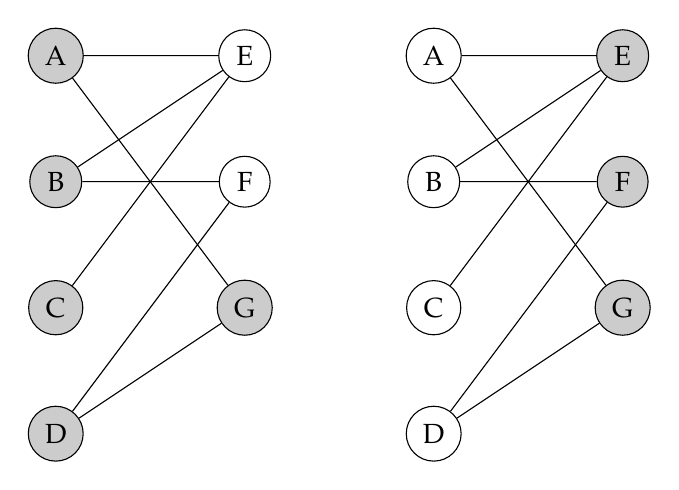
\begin{tikzpicture}[scale=.8,auto=left,every node/.style={circle,draw=black}]
		
		%left nodes
		\node[fill=black!20] (n1) at (1,10) {A};
		\node[fill=black!20] (n2) at (1,8) {B};
		\node[fill=black!20] (n3) at (1,6) {C};
		\node[fill=black!20] (n4) at (1,4) {D};

		%right nodes
		\node (n5) at (4,10) {E};
		\node (n6) at (4, 8) {F};
		\node[fill=black!20] (n7) at (4, 6) {G};
		
		%edges
		\draw (n1) -- (n5);
		\draw (n1) -- (n7);
		\draw (n2) -- (n5);
		\draw (n2) -- (n6);
		\draw (n3) -- (n5);
		\draw (n4) -- (n6);
		\draw (n4) -- (n7);

		%left nodes
		\node (m1) at (7,10) {A};
		\node (m2) at (7,8) {B};
		\node (m3) at (7,6) {C};
		\node (m4) at (7,4) {D};

		%right nodes
		\node[fill=black!20] (m5) at (10,10) {E};
		\node[fill=black!20] (m6) at (10, 8) {F};
		\node[fill=black!20] (m7) at (10, 6) {G};
		
		%edges
		\draw (m1) -- (m5);
		\draw (m1) -- (m7);
		\draw (m2) -- (m5);
		\draw (m2) -- (m6);
		\draw (m3) -- (m5);
		\draw (m4) -- (m6);
		\draw (m4) -- (m7);

		\end{tikzpicture}
		\caption{Examples of vertex covers.}
	\end{figure}
	You can convince yourself that the cover on the right is a minimum cover, i.e. there are no 
	vertex covers on this graph of size less than three. This brings us 
	to an important theorem, but we must first prove a lemma.

	\begin{lemma}
		Let $G=(U,V,E)$ be a bipartite graph. Let $M$ be a matching on $G$ and $C$ a vertex 
		cover on $G$ such that $|M| = |C|$. Then $M$ is a maximum matching and $C$ is a minimum 
		vertex cover.
	\end{lemma}

	\begin{proof}
		Let $M\'$ be a maximum matching on $G$ and $C\'$ a be a minimum vertex cover on $G$. 
		For each $(u,v)\in M\'$, $C\'$ must include either $u$ or $v$, which tells us that 
		$|M\'| \leq |C\'|$. We then have  
		\[
			|M|\leq |M\'| \leq |C\'| \leq |C|.
		\]
		Thus, if $|M| = |C|$ we have equalities above, which means that the size of a maximum 
		matching is equal to the size of a minimum covering.
	\end{proof}
	Before we prove the following theorem, we want to be able to talk about collections of 
	alternating paths, as it will be useful to us in discussing the methods of finding maximum 
	matchings on graphs.
	\begin{definition}
		Let $G = (U,V,E)$ be a bipartite graph, and $M$ a matching on $G$. An 
		\emph{alternating tree} with respect to $M$ is a tree which satisfies two 
		conditions:
		\begin{itemize}
			\item the tree contains exactly one unmatched $u\in U$. We call $u$ the 
				\emph{root} of the tree.
			\item all paths between the root and any other node in the tree are 
				alternating paths.
		\end{itemize}
	\end{definition}
	A graph with a corresponding alternating tree is shown in Figure 2.2.
	\begin{figure}[h]
		\centering
		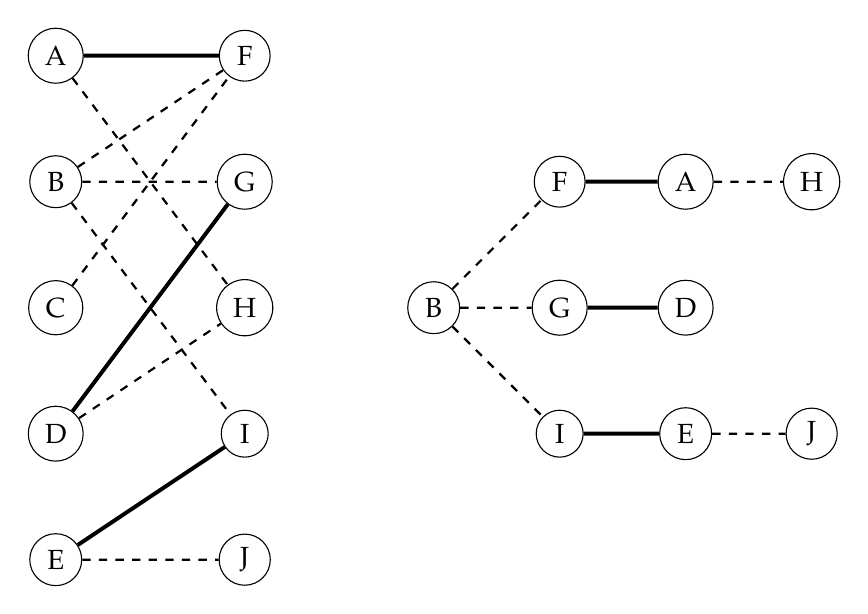
\begin{tikzpicture}[scale=.8,auto=left,every node/.style={circle,draw=black}]
		
		%left nodes
		\node (n1) at (1,10) {A};
		\node (n2) at (1,8) {B};
		\node (n3) at (1,6) {C};
		\node (n4) at (1,4) {D};
		\node (n5) at (1,2) {E};

		%right nodes
		\node (n6) at (4,10) {F};
		\node (n7) at (4,8) {G};
		\node (n8) at (4,6) {H};
		\node (n9) at (4,4) {I};
		\node (n10) at (4,2) {J};
		
		%edges
		\draw[line width=0.5mm] (n1) -- (n6);
		\draw[thick,dashed] (n1) -- (n8);
		\draw[thick,dashed] (n2) -- (n6);
		\draw[thick,dashed] (n2) -- (n7);
		\draw[thick,dashed] (n3) -- (n6);
		\draw[line width=0.5mm] (n4) -- (n7);
		\draw[thick,dashed] (n4) -- (n8);
		\draw[thick,dashed] (n2) -- (n9);
		\draw[line width=0.5mm] (n5) -- (n9);
		\draw[thick,dashed] (n5) -- (n10);

		%alternating tree
		\node (n11) at (7,6) {B};
		\node (n12) at (9,8) {F};
		\node (n13) at (9,6) {G};
		\node (n14) at (9,4) {I};
		\node (n15) at (11,8) {A};
		\node (n16) at (11,6) {D};
		\node (n17) at (11,4) {E};
		\node (n18) at (13,8) {H};
		\node (n20) at (13,4) {J};

		%tree edges
		\draw[thick,dashed] (n11) -- (n12);
		\draw[thick,dashed] (n11) -- (n13);
		\draw[thick,dashed] (n11) -- (n14);
		\draw[line width=0.5mm] (n12) -- (n15);
		\draw[line width=0.5mm] (n13) -- (n16);
		\draw[line width=0.5mm] (n14) -- (n17);
		\draw[thick,dashed] (n15) -- (n18);
		\draw[thick,dashed] (n17) -- (n20);
		\end{tikzpicture}
		\caption{Bipartite graph with matching (left) and corresponding alternating tree 
		rooted at vertex B (right).}
	\end{figure}

	\begin{theorem}{(K\H{o}nig-Egervary)}
		For any bipartite graph $G$, if $M$ is a maximum matching on $G$ and $C$ is a minimum 
		vertex cover  on $G$, then $|M| = |C|$.
	\end{theorem}
	\begin{proof}
		Let $G=(U,V,E)$ be a bipartite graph, and let $M$ be a maximum matching on $G$. 
		Furthermore, define
		\begin{align}
			F &:= \{u\in U\; |\; u \text{ unmatched}\}\\
			R &:= \{\text{all vertices connected to vertices in $F$ by alternating paths}\}.
		\end{align}
		Let $S = R\cap U$ and $T = R\cap V$. Let $N(S)$ be the set of all vertices 
		connected to elements of $S$ (i.e. the ``neighbors'' of $S$). Then we have the following:
		\begin{align*}
			&(1)\text{ Every vertex in $T$ is matched;}\\
			&(2)\ N(S) = T.
		\end{align*}
		The first claim comes from the fact that, if $M$ is a 
		maximum matching, then our alternating paths that start at a vertex in $F$ must have 
		an even length $\geq 2$. Otherwise, we would have an augmenting path, 
		which contradicts our assumption that $M$ is a maximum matching.
		The second claim comes from the fact that every node in $N(S)$ is connected to vertices 
		in $F$ by an alternating path. 

		Now, define $C := (U\setminus S)\cup T$. Every edge 
		in $G$ must have one of its endpoints in $C$. If not, then there would be an 
		edge with one endpoint in $S$ and one endpoint in $V\setminus T$, which contradicts 
		$N(S) = T$. Therefore $C$ is a vertex cover of $G$. Moreover, $|C| = |M|$, since for each 
		edge in $M$ we've included one of its endpoints in $C$ (the vertices we've chosen are 
		those in $N(S)$ and those in $U\setminus S$). Thus, by the previous lemma, $C$ is 
		a minimum covering.
	\end{proof}

	This theorem and lemma tell us that there is a deep relationship between maximum matchings and 
	minimum vertex covers on bipartite graphs. Subsequently, given a solution to a maximum matching 
	problem, we can turn it into a solution to a minimum vertex cover problem, and vice versa. Our 
	goal now is to generalize this concept.
\end{section}

\begin{section}{Duality Theory}
	We now turn to duality theory, which allows us to speak more generally about the relationships 
	between certain combinatorial problems that we are interested in solving.
	\begin{definition}
		Let the \emph{primal linear program} be the following linear program.
		\begin{alignat}{3}
			& \text{maximize } & \sum_{i=1}^{n} c_{i} x_{i}& \\
			& \text{subject to } \quad & \sum_{i=1}^{n} a_{ij} x_{i} & \leq b_{j}, & j & 
			= 1, \dots , m \\
					&& x_{i} & \geq 0, \quad & i & = 1, \dots, n.
		\end{alignat}		
		Then we define the \emph{dual linear program} of this primal linear program to be the 
		following linear program.
		\begin{alignat}{3}
			& \text{minimize } & \sum_{j=1}^{m} b_{j} y_{j}& \\
			& \text{subject to } \quad & \sum_{j=1}^{n} a_{ij} y_{j} & \geq c_{i}, & i & 
			= 1, \dots , m \\
					&& y_{j} & \geq 0, \quad & j & = 1, \dots, n.
		\end{alignat}		

		The dual of the dual is always the primal.
	\end{definition}
	In some settings we instead 
	have a minimization problem (the dual here) acting as the primal problem, while the maximization 
	problem is actually the dual. Ultimately, it does not matter which one we call the dual and
	which one we call the primal; what matters is how they relate to each other. 
	Let us introduce some 
	notation. First, let us denote the primal maximization problem by $\Gamma$, and 
	the dual minimization problem by $\Omega$. For a given linear program, we denote 
	an optimal solution by $\mathbf{OPT}$, by which we mean the value that optimizes the objective 
	function and satisfies the linear constraints. Naturally, we want to know how solutions to 
	linear programs that are primal-dual to each other relate.

	\begin{theorem}{(Weak duality)}
		If the primal linear program (in maximization form) and the dual (in minimization 
		form) are both feasible, then 
		\[
			\mathbf{OPT}(\Gamma) \leq \mathbf{OPT}(\Omega).
		\]
	\end{theorem}

	\begin{proof}
		Suppose that $\mathbf{x} = (x_1, x_2,\dots,x_n)$ is a feasible solution to $\Gamma$, and 
		$\mathbf{y} = (y_1, y_2, \dots y_m)$ is a feasible solution to $\Omega$. 
		So $\mathbf{OPT}(\Gamma) = \sum_{i=1}^{n} c_i x_i$ and 
		$\mathbf{OPT}(\Omega) = \sum_{j=1}^{m} b_j y_j$.
		Because 
		$\mathbf{y}$ is dual feasible and all $x_i$ and $y_j$ are nonnegative, we have 
		\[
			\sum_{j=1}^{m} b_j y_j \geq \sum_{j=1}^{m}\left(\sum_{i=1}^{n} a_{ij}x_i\right) 
			y_j.
		\]
		Similarly, we have that 
		\[
			\sum_{i=1}^{n} c_i x_i \leq \sum_{i=1}^{n}\left(\sum_{j=1}^{m} a_{ij} y_j\right) 
			x_i.
		\]
		Note that by rearranging terms, we have the following equality:
		\[
			\sum_{i=1}^{n}\left(\sum_{j=1}^{m} a_{ij} y_j\right) 
			x_i =
			\sum_{j=1}^{m}\left(\sum_{i=1}^{n} a_{ij}x_i\right) 
			y_j,
		\]
		which shows that 
		\[
			\sum_{i=1}^{n} c_i x_i \leq 
			\sum_{i=1}^{n}\left(\sum_{j=1}^{m} a_{ij} y_j\right) 
			x_i =
			\sum_{j=1}^{m}\left(\sum_{i=1}^{n} a_{ij}x_i\right) 
			y_j \leq 
			\sum_{j=1}^{m} b_j y_j,
		\]
		so $\mathbf{OPT}(\Gamma) \leq \mathbf{OPT}(\Omega)$.
	\end{proof}
	What's surprising is the following theorem.

	\begin{theorem}{(Strong duality)}
		Given two linear programs $\Gamma$ and $\Omega$ that are duals of each other, if one is 
		feasible and bounded, then so is the other. Additionally, 
		\[
			\mathbf{OPT}(\Gamma) = \mathbf{OPT}(\Omega).
		\]
	\end{theorem} 
	In Chapter 4 we will use duality theory to get necessary and sufficient conditions for 
	$\mathbf{OPT}(\Gamma) = \mathbf{OPT}(\Omega)$, which will give us \textbf{Theorem 2.6}.
	Our goal now is to use facts about duality to better understand the relationships between 
	our combinatorial optimization problems.

\begin{subsection}{Maximum-Matching Duality}
	Let us formulate the maximum matching as a linear program. Our goal is to maximize the number 
	of edges in our matching. Let us define a set of variables $x_{uv}$, one for each $(u,v)\in E$. 
	These will be the unknowns in the linear program. We will use these to define a subset of 
	edges as follows: when $x_{uv} = 1$, we will say that $(u,v)$ is included in that subset; 
	when $x_{uv} = 0$, we will say that $(u,v)$ is excluded from that subset. Since we are trying 
	to construct a matching on our graph, we need the constraints that ensure no edge is incident to 
	more than one vertex in the matching; otherwise, the matching would be invalid. For a fixed 
	vertex $u\in U$, the number of edges in the matching incident 
	to $u$ is given by $\sum_{v\in V} x_{uv}$. So we want this to be less than or equal to one. 
	Similarly, for any vertex $v\in V$, we want $\sum_{u\in U} x_{uv}$ to be less than or equal to 
	one. This gives us the following linear program:
	\begin{alignat}{3}
		& \text{maximize } & \sum_{u,v} x_{uv}& \\
		& \text{subject to } \quad & \sum_{v} x_{uv} & \leq 1, & \quad \text{for all } u\in U& \\
				     &\quad & \sum_{u} x_{uv} & \leq 1, & \quad \text{for all } v\in 
				     V & \\
				&& x_{uv} & \in \{0,1\}.
	\end{alignat}

	What we have presented here is an $\emph{integer}$ linear program, since we've restricted our 
	$x$ variables to be integers. In general, solving integer linear programs is NP-hard. However, 
	in this case it is well known that this linear program attains an integer solution at extreme 
	points
	(see Birkhoff \cite{birkhoff1946} and von Neumann \cite{vN53})
	of the polyhedron solution space, so we can drop the integrality requirements and just say 
	$x_{uv} \geq 0$.

	Now let us try and construct the dual of this linear program. To do this we will need a variable 
	$y_u$ for each vertex $u$. Similarly, we need a variable $y_v$ for each vertex $v$. Our 
	objective will be to minimize over the sum of these $y_u$ and $y_v$. Since our coefficient on 
	$x_{uv}$
	in the primal is the constant vector one, our only constraint will be that $y_u + y_v \geq 1$. 
	This gives us the dual linear program:
	\begin{alignat}{3}
		& \text{minimize } & \sum_{u\in U} y_u + \sum_{v\in V} y_v& \\
		& \text{subject to } \quad & y_u + y_v & \geq 1, & \quad \text{for all } 
					(u,v)\in E & \\
				    && y_u,y_v & \geq 0.
	\end{alignat}
	This dual problem tells us that each edge must be ``covered'' by at least one of its incident 
	vertices. This is exactly the vertex cover problem! So, for unweighted bipartite graphs, the 
	linear programs for maximum matchings and minimum vertex covers are duals of each other. 
	We will use this insight to construct our algorithms for solving the maximum matching problem. 

	There is another variant of the maximum matching problem called the 
	\emph{maximum weight matching problem}. In this 
	version, we are given a bipartite graph with non-negative edge weights $w_{uv}$ for all 
	edges $(u,v)\in E$. Instead of trying to maximize the number of edges in the matching, the goal 
	is to find a matching $M$ such that $\sum_{(u,v) \in M} w_{uv}$, or the total ``weight'' of the 
	matching, is greater than the weight of any other matching. 
	We can easily encode this problem by making 
	a slight modification to our linear program from before. The primal is given by the following 
	linear program:
	\begin{alignat}{3}
		& \text{maximize } & \sum_{u,v} w_{uv}x_{uv}& \\
		& \text{subject to } \quad & \sum_{v} x_{uv} & \leq 1, & \quad 
					\text{for all } u\in U& \\
				     &\quad & \sum_{u} x_{uv} & \leq 1, & \quad 
				     	\text{for all } v\in V & \\
				&& x_{uv} & \geq 0.
	\end{alignat}
	Then the dual is given by:
	\begin{alignat}{3}
		& \text{minimize } & \sum_{u} y_u + \sum_v y_v& \\
		& \text{subject to } \quad & y_u + y_v & \geq w_{uv}, & \quad \text{for all } 
					(u,v)\in E & \\
				    && y_u,y_v & \geq 0.
	\end{alignat}
	The dual is a sort of weighted vertex cover. One way to think about it is that each edge 
	has a ``cost'' given by $w_{uv}$, and each of its endpoints (vertices) must pool ``money'' 
	in order 
	to pay at least that cost. So instead of edges being covered or not covered, there is a certain 
	``amount'' that they have to be covered.

	These two problems, the maximum weight matching and the minimum weight vertex cover, are the 
	problems that the Hungarian algorithm solves, which we discuss in Chapter 3. For now, we digress 
	and discuss the max-flow min-cut theorem, as an ode to students who have taken a course in 
	algorithms.
\end{subsection}

\begin{subsection}{The Max-Flow Min-Cut Theorem}
	Here we demonstrate that a common problem discussed in algorithms courses, and a quite 
	amazing theorem, is really a special case of what we have been discussing. 
	We first recall the definition of a flow network.
	\begin{definition}
		A \emph{flow network} $G = (V,E)$ is a directed graph in which each edge $(u,v)\in E$ 
		has an assigned \emph{capacity} $c_{uv} \geq 0$. Furthermore, there are two 
		distinguished vertices in $V$, a source $s$ and a sink $t$. 
		We assume that every $v\in V$ lies in some path $s\to \cdots \to v\to \cdots \to t$.
	\end{definition}
	Given a flow network, we can define a function on the network.
	\begin{definition}
		Let $G = (V,E)$ be a flow network. A \emph{flow} on $G$ is a function $f: V\times V \to 
		\R$ that satisfies the following:
		\begin{itemize}
			\item Capacity constraint: For all $u,v\in V$, $0\leq f(u,v) \leq 
				c_{uv}$.
			\item Flow conservation: For all $u\in V\setminus \{s,t\}$, we have 
				\[
					\sum _{v\in V} f(v,u) = \sum_{v\in V} f(u,v).
				\]
				This says that, for all vertices $v$ except our source and sink, the 
				flow out of $v$ is equal to the flow into $v$. 
		\end{itemize}
		We define the value of the flow to be $val(f) = \sum_{v\in V} f(s,v) - \sum_{v\in V} 
		f(v,s)$, which is just the flow out of our source minus the flow into our source.
	\end{definition}
	\begin{figure}[h]
		\centering
		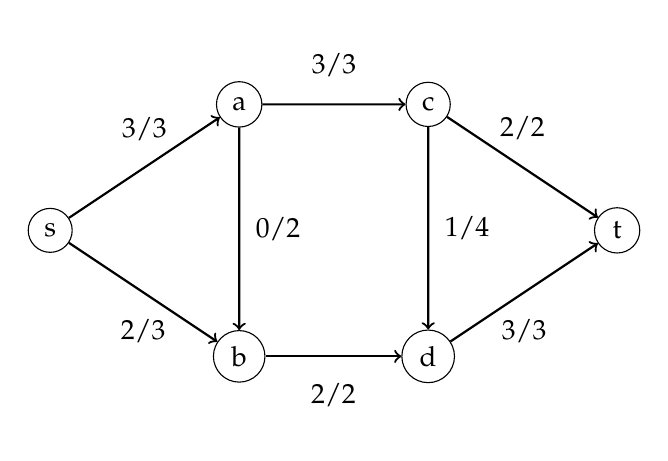
\begin{tikzpicture}[scale=.8,auto=left,every node/.style={circle,draw=black}]
			\node (n1) at (3,3) {s};
			\node (n2) at (6,5) {a};
			\node (n3) at (6,1) {b};
			\node (n4) at (9,5) {c};
			\node (n5) at (9,1) {d};
			\node (n6) at (12,3) {t};

			\draw[->,thick] (n1) -- node[draw=none, above] {3/3} ++ (n2);
			\draw[->,thick] (n1) -- node[draw=none, below] {2/3} ++ (n3);
			\draw[->,thick] (n2) -- node[draw=none, right] {0/2} ++ (n3);
			\draw[->,thick] (n2) -- node[draw=none, above] {3/3} ++ (n4);
			\draw[->,thick] (n3) -- node[draw=none, below] {2/2} ++ (n5);
			\draw[->,thick] (n4) -- node[draw=none, right] {1/4} ++ (n5);
			\draw[->,thick] (n4) -- node[draw=none, above] {2/2} ++ (n6);
			\draw[->,thick] (n5) -- node[draw=none, below] {3/3} ++ (n6);
		\end{tikzpicture}
		\caption{Flow network with maximum flow of 5. Notation: $X/Y$ means an edge has capacity 
		$Y$ and flow $X$, given by the flow function.}
	\end{figure}
	In Figure 2.3, (from Cormen, Leiserson, Rivest, and Stein \cite{cormen2009introduction}) 
	we have a flow network with a corresponding flow. For example, the capacity 
	of the edge $(s,b)$ is $3$, and our flow function in sending a flow of value $2$ through 
	this edge.

	The problem, as demonstrated in a typical algorithms course, is to find a maximum flow from $s$ 
	to $t$. This is done using a method developed by Ford and Fulkerson which looks for augmenting 
	paths in the residual graph (essentially the subgraph where the flows $f(u,v) < c_{uv}$. 
	The reader should refer to Cormen, Leiserson, Rivest, and Stein 
	\cite{cormen2009introduction} for a more detailed treatment. Now, we recall the definition 
	of a cut in a flow network.
	\begin{definition}
		An $s-t$ \emph{cut} $(S,T)$ of a flow network $G=(V,E)$ is a partition of $V$ into 
		sets $S$ and $T = V\setminus S$ such that $s\in S$ and $t\in T$. Given a flow $f$, the 
		\emph{net flow} $f(S,T)$ across the cut $(S,T)$ is defined as 
		\[
			f(S,T) = \sum_{u\in S} \sum_{v\in T} f(u,v) - \sum_{u\in S} \sum_{v\in T} 
			f(v,u).
		\]
		Finally, the \emph{capacity} of the cut is defined as $c(S,T) = 
		\sum_{u\in S} \sum_{v\in T} c(u,v)$. A \emph{minimum cut} has capacity less than or 
		equal to all other cuts in the network.
	\end{definition}
	One of the coolest and most surpising theorems in an algorithms course is that, given a flow 
	network $G$, the value of the maximum flow on $G$ is equal to the capacity of the minimum 
	$s-t$ cut of $G$.

	Our goal now is to build up to this same theorem using the tools developed in this chapter,
	following the treatment given by Vazirani \cite{vazirani2002approximation}. 
	We will first give a linear program for the 
	maximum flow problem. To make things simpler, let us introduce an arc of infinite capacity 
	from the sink $t$ to the source $s$; this converts this to a \emph{circulation} problem, 
	with the objective to maximize the flow $f(t,s)$. This allows us to enforce flow conservation 
	at $s$ and $t$ as well, which makes the corresponding linear program simpler. The linear 
	program is as follows:
	\begin{alignat}{3}
		& \text{maximize } & f(t,s)\\
		& \text{subject to } & f(u,v) &\leq c_{uv}, &\quad (u,v)\in E\\ 
				     && \sum_{v:(v,u)\in E} f(v,u) & \leq \sum_{v:(u,v)\in E} f(u,v), &
				     	\quad u\in V &\\
				     && f(u,v) &\geq 0. &\quad (u,v)\in E &
	\end{alignat}
	It is not immediately obvious why the second set of inequalities implies flow conservation; 
	at first glance all 
	it seems to say is that for each $u$, the total flow into $u$ is at most the total flow out 
	of $u$. However, note that if this holds for all $u$, we in fact have equality of incoming and 
	outgoing flow, since a deficit of flow at some $u$ implies a flow surplus at some $v$. So 
	this does in fact give us conservation of flow. 
	
	Now we want to find the dual of this program. 
	Our sense (hopefully) is that the dual will somehow relate to minimum cuts, given the 
	foreshadowing of the previous section. Let's see! We introduce variables $d_{uv}$ and $p_u$ for 
	inequalities (2.24) and (2.25), respectively. Then the dual linear program is as follows:
	\begin{alignat*}{3}
		& \text{minimize } & \sum_{(u,v)\in E} c_{uv} d_{uv}& \\
		& \text{subject to } \quad & d_{uv} - p_u + p_v & \geq 0, & \quad 
					\text{for all }(u,v)\in E & \\
				    && p_s - p_t & \geq 1, & \\
				    && d_{uv} & \geq 0, & \quad \text{for all }(u,v) \in E & \\
				    && p_u,\ p_v & \geq 0.
	\end{alignat*}
	It is known that extreme point solutions to these linear programs take on values zero or one at 
	each coordinate. Let us now consider an optimal dual solution $(\mathbf{d}^{*},\mathbf{p}^{*})$. 
	First, in order to satisfy $p_s^{*} - p_{t}^{*} \geq 1$ with zero/one values, it must 
	be the case that $p_s^{*} = 1$ and $p_t^{*} = 0$. This motivates an $s-t$ cut $(S,T)$ 
	with $S$ consisting 
	of vertices with value one, and $T$ the vertices with value zero. For an edge $(u,v)$ such that 
	$u\in S$ and $v\in T$, we have that $p_u^{*} = 1$ and $p_v^{*} = 0$, so by the first constraint 
	$d_{uv}^{*} = 1$. This means that for any edge $(u,v)$ in the cut, the corresponding 
	$d_{uv}^{*} = 1$. Note that any other $d_{uv}^{*}$ where $(u,v)$ is not in the cut can take value 
	zero without violating the constraints (in fact we want these $d_{uv}^{*}=0$ since we are 
	minimizing our objective function). Thus the objective function's value is equal to the capacity 
	of this $s-t$ cut, which must be a minimum cut. Strong duality tells us that this corresponds 
	to the value of $f(t,s)$ in the primal linear program. 
	
	To make this clear, let us look back at our flow network in Figure 2.3. 
	We expect that, given our discussion of the dual, we should be able to find a cut 
	$(S,T)$ of the flow network that has value five. 
	Moreover, this cut $(S,T)$ should be such that $S$ consists of vertices with value one, 
	and $T$ consists of vertices with value zero. 
	We know that we must set $p_s = 1$ and $p_t = 0$. This gives us the following dual solution 
	shown in Figure 2.4.
	\begin{figure}[h]
		\centering
		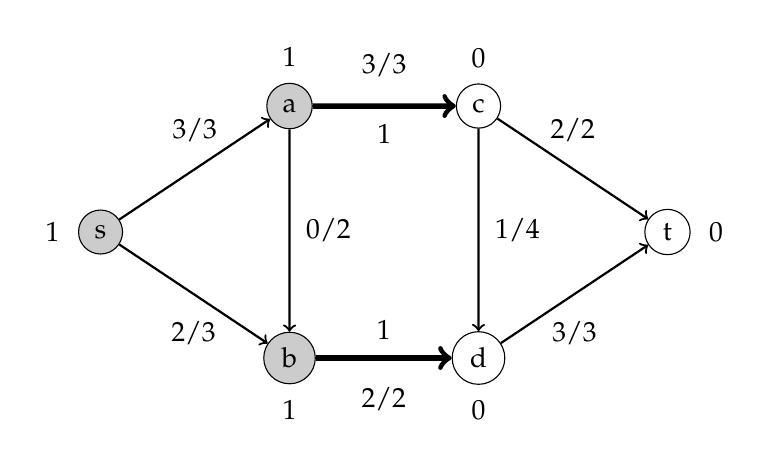
\begin{tikzpicture}[scale=.8,auto=left,every node/.style={circle,draw=black}]
			\node [fill=black!20, label=left:{1}] (n1) at (3,3) {s};
			\node [fill=black!20, label=above:{1}] (n2) at (6,5) {a};
			\node [fill=black!20, label=below:{1}] (n3) at (6,1) {b};
			\node [label=above:{0}] (n4) at (9,5) {c};
			\node [label=below:{0}] (n5) at (9,1) {d};
			\node [label=right:{0}] (n6) at (12,3) {t};

			\draw[->,thick] (n1) -- node[draw=none, above] {3/3} ++ (n2);
			\draw[->,thick] (n1) -- node[draw=none, below] {2/3} ++ (n3);
			\draw[->,thick] (n2) -- node[draw=none, right] {0/2} ++ (n3);
			\draw[->,line width=0.7mm] (n2) -- node[draw=none, above] {3/3} 
			node[draw=none, below] {1} ++ (n4);
			\draw[->,line width=0.7mm] (n3) -- node[draw=none, below] {2/2} 
			node[draw=none, above] {1} ++ (n5);
			\draw[->,thick] (n4) -- node[draw=none, right] {1/4} ++ (n5);
			\draw[->,thick] (n4) -- node[draw=none, above] {2/2} ++ (n6);
			\draw[->,thick] (n5) -- node[draw=none, below] {3/3} ++ (n6);
		\end{tikzpicture}
		\caption{Flow network with corresponding dual solution (bold edges are the edges in our 
		cut).}
	\end{figure}

	In this figure the $s-t$ cut corresponds to the sets $S= \{\mbox{s},\mbox{a},\mbox{b}\}$ and 
	$T = \{\mbox{c},\mbox{d},\mbox{t}\}$; the 
	edges in the cut are the bold edges $(\mbox{a},\mbox{c})$ and $(\mbox{b},\mbox{d})$. 
	So the capacity of the cut is five, 
	which is what we'd expect. In order to make the figure readable, we leave out our dual labeling 
	on edges that are not in the cut (their label is ``0'' anyways). Edges in the cut have label 
	``1'', as shown in the figure. Note that our dual labeling of edges and vertices in this flow 
	network satisfies our dual constraints.

	Thus, we have given an alternative formulation of the max-flow min-cut relationship using 
	linear programs. In the next chapter, we present the main algorithm of this thesis, the 
	Hungarian algorithm, which is interesting in and of itself, and also as a tool to motivate 
	general primal-dual algorithms.
\end{subsection}
\end{section}


\chapter{The Hungarian algorithm}

In this chapter, we present a comprehensive look at the Hungarian algorithm. The algorithm relies on 
some interesting techniques, which we spell out carefully. Ultimately, we show how this algorithm 
solves its associated primal and dual linear programs -- the maximum weight matching and 
the minimum weight vertex cover problems, respectively.

\begin{section}{Preliminaries}
	In this section, we use the motivation of the linear programs to develop an algorithm for 
	simultaneously solving the maximum weight matching and minimum weight vertex cover problems. 
	Our algorithm works by taking every exposed vertex on the left, and from each such 
	vertex building a collection of alternating paths. For our graphs $G = (U,V,E)$ we will assume 
	$|U| = |V|$.
	
	Let us remind ourselves what the primal-dual linear programs
	motivate. We want to minimize $\sum w_{uv}$ and maximize $(\sum_u y_u + \sum_v y_v)$. Moreover, 
	we want optimal solutions (i.e. $\sum w_{uv} = \sum_u y_u + \sum_v y_v$). For our primal, we are 
	keeping track of edge weights. For the dual, we will be keeping track of a ``labeling'' on 
	vertices, given by the $y_u$ and $y_v$ values. We define what a labeling is now.
	\begin{definition}
		A \emph{vertex labeling} on a weighted bipartite graph $G = (U,V,E)$ is a function 
		$l: U\cup V \to \N$. We call a labeling \emph{feasible} if for all $u\in U$ and 
		$v\in V$, $l(u) + l(v) \geq w_{uv}$.
	\end{definition}
	This labeling corresponds to our dual variables; a feasible labeling is a feasible dual 
	solution. It will be helpful for us to look at a certain subset of our graph where the labeling 
	is exact (i.e. where $l(u) + l(v) - w_{uv} = 0$).
	\begin{definition}
		The \emph{equality subgraph} of $G = (U,V,E)$ is the graph $G_l = (U,V,E_l)$, 
		where 
		\[
			E_l = \{(u,v)\ :\ l(u) + l(v) = w_{uv}\}.
		\]
	\end{definition}
	In Figure 3.1 we show a bipartite graph along with its corresponding equality graph.
	\begin{figure}[h]
		\centering
		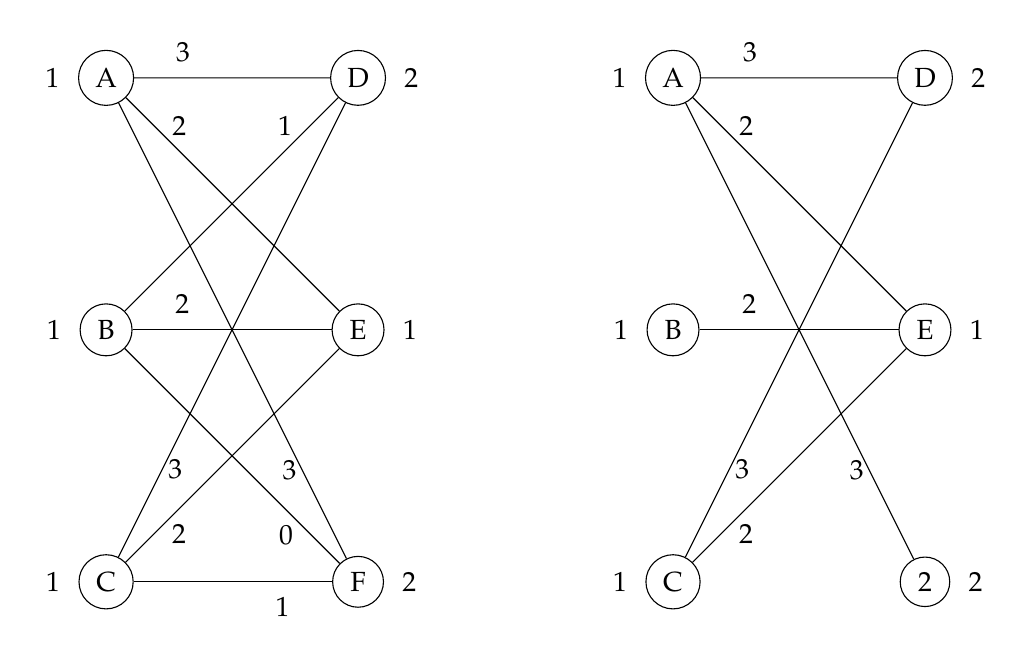
\begin{tikzpicture}[scale=.8,auto=left,every node/.style={circle,draw=black}]
			%left nodes
			\node [label=left:{1}] (n1) at (1,10) {A};
			\node [label=left:{1}] (n2) at (1,6) {B};
			\node [label=left:{1}] (n3) at (1,2) {C};

			%right nodes
			\node [label=right:{2}] (n4) at (5,10) {D};
			\node [label=right:{1}] (n5) at (5,6) {E};
			\node [label=right:{2}] (n6) at (5,2) {F};

			%edges
			\draw (n1) -- node[near start,draw=none,above] {3} ++(n4);
			\draw (n1) -- node[near start,draw=none,above] {2} ++(n5);
			\draw (n1) -- node[near end,draw=none,below] {3} ++(n6);

			\draw (n2) -- node[near end,draw=none,above] {1} ++(n4);
			\draw (n2) -- node[near start,draw=none,above] {2} ++(n5);
			\draw (n2) -- node[near end,draw=none,below] {0} ++(n6);

			\draw (n3) -- node[near start,draw=none,below] {3} ++(n4);
			\draw (n3) -- node[near start,draw=none,below] {2} ++(n5);
			\draw (n3) -- node[near end,draw=none,below] {1} ++(n6);


			%left nodes
			\node [label=left:{1}] (n7) at (10,10) {A};
			\node [label=left:{1}] (n8) at (10,6) {B};
			\node [label=left:{1}] (n9) at (10,2) {C};

			%right nodes
			\node [label=right:{2}] (n10) at (14,10) {D};
			\node [label=right:{1}] (n11) at (14,6) {E};
			\node [label=right:{2}] (n12) at (14,2) {2};

			%edges
			\draw (n7) -- node[near start,draw=none,above] {3} ++(n10);
			\draw (n7) -- node[near start,draw=none,above] {2} ++(n11);
			\draw (n7) -- node[near end,draw=none,below] {3} ++(n12);

			\draw (n8) -- node[near start,draw=none,above] {2} ++(n11);

			\draw (n9) -- node[near start,draw=none,below] {3} ++(n10);
			\draw (n9) -- node[near start,draw=none,below] {2} ++(n11);
		\end{tikzpicture}
		\caption{A weighted bipartite graph (left) and its corresponding equality subgraph
		(right).}
	\end{figure}
	\begin{theorem}{(Kuhn-Munkres)}
		If $l$ is a feasible labeling and $M$ is a perfect matching in $G_l$ then $M$ is a 
		maximum weight matching.
	\end{theorem}

	\begin{proof}
		Let $M\'$ be a perfect matching in $G$. Since every $u\in U\cup V$ is included 
		in exactly one edge in $M\'$, then 
		\[
			\sum_{(u,v)\in M\'} w_{uv} \leq \sum_{(u,v)\in M\'} (l(u)+l(v)) = 
			\sum_{z\in U\cup V} l(z).
		\]
		This says that the sum of our label values is an upper bound on the weight of any 
		perfect matching.

		Now suppose that $M$ is a perfect matching in $G_l$. Then 
		\[
			\sum_{(u,v)\in M} w_{uv} = \sum_{z\in U\cup V} l(z).
		\]
		So $\sum_{(u,v)\in M\'} w_{uv} \leq \sum_{(u,v)\in M} w_{uv}$, 
		meaning that $M$ must be a maximum weight matching.
	\end{proof}
	This theorem tells us that if we can give an algorithm for finding a perfect matching in the 
	equality subgraph (if such a matching exists), then we can find a maximum weight matching in the 
	graph. To do this, we will first define a few terms. 

	As in Chapter 2, let $R$ be the set of vertices reachable from unmatched vertices in $U$ via 
	alternating paths, 
	and let $S:=R\cap U$, $T:=R\cap V$. We will use these sets to construct our collection of 
	alternating trees.
	
	Now, consider a feasible labeling $l$ on a graph $G = (U,V,E)$ and set 
	\[
		\delta := \min_{u\in S,\ v\notin T} \{l(u) + l(v) - w_{uv} \}.
	\]
	We define a new labeling $l^{'}$ as follows:
		\[
			l\' (z) = 
			\begin{cases}
				l(z) - \delta &\text{ if } z\in S \\
				l(z) + \delta &\text{ if } z\in T \\
				l(z) &\text{ otherwise.}
			\end{cases}
		\]
	\begin{lemma}
		The labeling $l^{'}$ as defined above is a feasible labeling.
	\end{lemma}

	\begin{proof}
		To show this labeling is feasible, we must show that for any edge $(u,v)$, 
		$l^{'}(u) + l^{'}(v) \geq w_{uv}$. For $u\in U$, $v\in V$, there are four possibilities:
		\begin{enumerate}
			\item If $u\in S$ and $v\in T$ then $l\' (u) + l\' (v) = l(u) + l(v)$. This 
				is because $l^{'}(u) = l(u) - \delta$ and $l^{'}(v) = l(v) + \delta$. 
			\item If $u\notin S$ and $v\notin T$, $l\' (u) = l(u)$ and $l\' (v) = l(v)$, 
				so $l\' (u) + l\' (v) = l(u) + l(v)$.
			\item If $u\in S$ and $v\notin T$, $l\' (u)=l(u) - \delta$ and $l\' (v) = l(v)$. 
				We know $\delta = \min_{u\in S,v\notin T} \{l(u) + l(v) - w_{uv}\}$, 
				which means $\delta \leq l(u) + l(v) - w_{uv}$, and thus 
				$l\' (u) + l\' (v) \geq w_{uv}$.
			\item If $u\notin S$ and $v\in T$, $l\' (u) = l(u)$ and $l\' (v) = l(v) + 
				\delta$. So we get $l^{'}(u) + l^{'}(v) = l(u) + l(v) + \delta \geq 
				w_{uv}$.
		\end{enumerate}
	\end{proof}
	We also need to show that this labeling increases the size of our equality graph.
	\begin{lemma}
		Given an initial feasible labeling $l$ and the labeling $l^{'}$, the following 
		hold:
		\begin{enumerate}
			\item If $(u,v)\in E_l$ and $u\in S$, $v\in T$, then $(u,v)\in E_{l^{'}}$. 
			\item If $(u,v)\in E_l$ and $u\notin S$, $v\notin T$, then $(u,v)\in 
				E_{l^{'}}$.
			\item If $u\notin S$ and $v\in T$, then $(u,v)\notin E_l$.
			\item If $u\in S$ and $v\notin T$ then $(u,v)\notin E_l$.
			\item There exists some $(u,v)$ such that $u\in S$ and $v\notin T$, and 
				$(u,v)\in E_{l^{'}}$. 
		\end{enumerate}
	\end{lemma}
	\begin{proof}
		The claims (1) and (2) are made clear by the previous lemma. \\
		To prove claim (3), suppose towards a contradiction that $(u,v)\in E_l$ with 
		$u\notin S$ and $v\in T$. This means that since $v\in T$, $u$ is reachable by some 
		alternating path in $R$, hence $u\in S$, which is a contradiction.\\
		Part (4) follows from the fact that if $u\in S$ and $(u,v)\in E_l$, then $v$ is 
		reachable by an alternating path in $R$, hence $v\in T$, which is a contradiction.\\
		To see (5), note that there is some edge $(u,v)$ with 
		$u\in S$, $v\notin T$ such that $\delta = l(u) + l(v) - w_{uv}$, so when we take 
		$l\' (u) = l(u) - \delta$ and $l\' (v) = l(v)$, we get 
		\begin{align*}
			l\' (u) + l\' (v) - w_{uv} &= l(u) - \delta + l(v) - w_{uv} \\
						   &= l(u) + l(v) - w_{uv} - \delta \\
						   &= \delta - \delta \\
						   &= 0.
		\end{align*}
		This is exactly what it means for an edge $(u,v)$ to be in $E_l$. Hence $E_l \subset 
		E_{l^{'}}$. 
	\end{proof}

	\begin{theorem}
		$|E_l| < |E_{l^{'}}|$.
	\end{theorem}

	The proof of this theorem follows from the previous lemma, as we showed that 
	$E_l \subset E_{l^{'}}$.
\end{section}
\begin{section}{The Hungarian Algorithm}
	We now look at the Hungarian method for finding maximum-weight matchings on bipartite graphs. 
	This method was originally developed by Kuhn and Munkres, who named it in honor of the Hungarian 
	mathematicians K\H{o}nig and Egervary. The algorithm is shown in Figure 3.2.
	\begin{figure}[h]
	\begin{center}
		\begin{minipage}{3in}
			\begin{codebox}
				\Procname{$\proc{Hungarian-Max-Assign} (U,V,E,w)$}
				\li $l_u := \max_{v} c_{uv}$
				\li $l_v := 0$
				\li Repeat the following:
				\li \quad $M := $ $\proc{Max-Card-Matching} (U,V,G_l)$
				\li \quad \If $M$ is a perfect matching in $G_l$
				\li \quad	\Then 
				    \quad		\Return $M$
				    \quad	\End
				\li \quad $R := $ $\proc{Alt-Path-Reachable} (U,V,E_l,M)$
				\li \quad $l :=$ $\proc{Label-Update} (R,U,V,E,w,l)$
			\end{codebox}
		\end{minipage}
	\end{center}
		\caption{The Hungarian Algorithm}
	\end{figure}

	The correctness of the algorithm follows from the lemma and theorem. Note that our labeling $l$ 
	remains feasible by Lemma 3.4, and the equality graph increases in size by Lemma 3.5. This tells 
	us that, assuming our graph $G$ has a perfect matching, one will eventually be found by this 
	algorithm. Since this perfect matching will be in $G_l$, Theorem 3.3 tells us that our final 
	matching $M$ will be of maximum weight.

	We now provide an example of this algorithm. This example is due to Golin \cite{hknotes}.
	\begin{figure}[h]
		\centering
		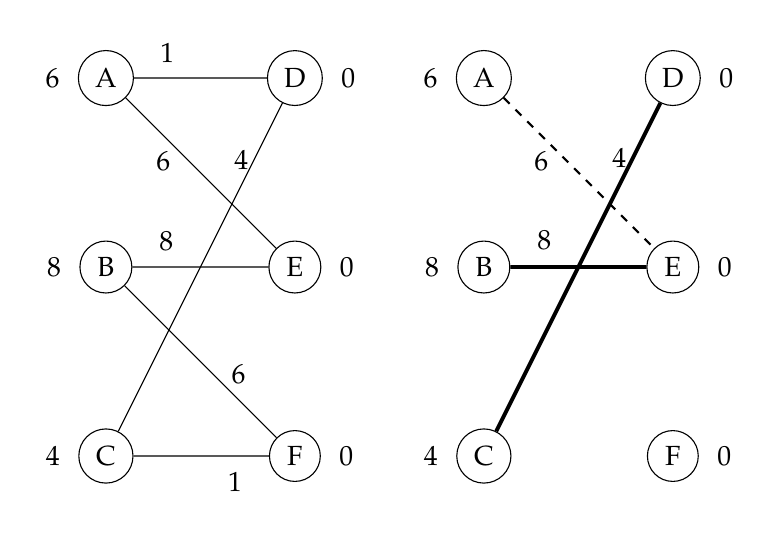
\begin{tikzpicture}[scale=.8,auto=left,every node/.style={circle,draw=black}]

			%left nodes
			\node [label=left:{6}] (n1) at (1,10) {A};
			\node [label=left:{8}] (n2) at (1,7) {B};
			\node [label=left:{4}] (n3) at (1,4) {C};

			%right nodes
			\node [label=right:{0}] (n4) at (4,10) {D};
			\node [label=right:{0}] (n5) at (4,7) {E};
			\node [label=right:{0}] (n6) at (4,4) {F};

			%edges
			\draw (n1) -- node[near start, draw=none, above] {1} ++ (n4);
			\draw (n1) -- node[near start, draw=none, below] {6} ++ (n5);
			\draw (n2) -- node[near start, draw=none, above] {8} ++ (n5);
			\draw (n2) -- node[near end, draw=none, above] {6} ++ (n6);
			\draw (n3) -- node[near end, draw=none, above] {4} ++ (n4);
			\draw (n3) -- node[near end, draw=none, below] {1} ++ (n6);

			
			
			%left nodes
			\node [label=left:{6}] (m1) at (7,10) {A};
			\node [label=left:{8}] (m2) at (7,7) {B};
			\node [label=left:{4}] (m3) at (7,4) {C};

			%right nodes
			\node [label=right:{0}] (m4) at (10,10) {D};
			\node [label=right:{0}] (m5) at (10,7) {E};
			\node [label=right:{0}] (m6) at (10,4) {F};
			
			%edges
			\draw[thick,dashed] (m1) -- node[near start, draw=none, below] {6} ++ (m5);
			\draw[line width=0.5mm] (m2) -- node[near start, draw=none, above] {8} ++ (m5);
			\draw[line width=0.5mm] (m3) -- node[near end, draw=none, above] {4} ++ (m4);
		\end{tikzpicture}
		\caption{Bipartite graph (left) and corresponding equality graph (right) with initial 
		matching}
	\end{figure}
	Our initial matching is $M = \{(\mbox{B},\mbox{E}), (\mbox{C},\mbox{D})\}$ (see Figure 3.3). 
	Note that the current state of 
	the graph is 
	primal-dual feasible. This matching $M$ is not perfect in $G_l$. The unmatched vertices in $U$ 
	consists of a single member, $\mbox{A}$, meaning our algorithm chooses $\mbox{A}$ to add to $R$. 
	So we have 
	$S=\{\mbox{A}\}$ and $T=\{\mbox{E}\}$ since $\mbox{E}$ is reaches to $\mbox{A}$ via the single 
	path. The vertex $\mbox{E}$ is matched, so we grow our alternating tree as follows: 
	$R := R\cup \{\mbox{B}\} = \{\mbox{A},\mbox{B}\}$, 
	$T := T\cup \{\mbox{E}\} = \{\mbox{E}\}$. At this point we adjust our labeling.
	Calculate $\delta = \min _{u\in S,v\notin T} \{l(u) + l(v) - w_{uv}\} = 2$ from edge 
	$(\mbox{B},\mbox{F})$. 
	Our new equality graph is shown in Figure 3.4.
	\begin{figure}[H]
		\centering
		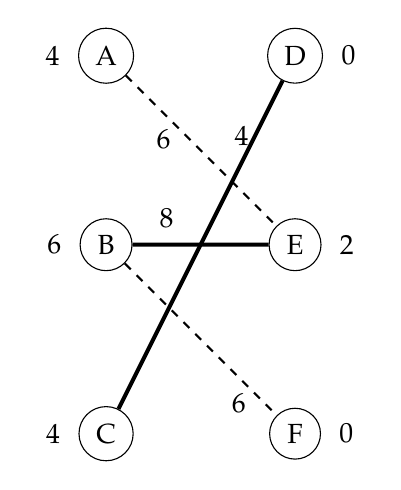
\begin{tikzpicture}[scale=.8,auto=left,every node/.style={circle,draw=black}]
			%left nodes
			\node [label=left:{4}] (m1) at (7,10) {A};
			\node [label=left:{6}] (m2) at (7,7) {B};
			\node [label=left:{4}] (m3) at (7,4) {C};

			%right nodes
			\node [label=right:{0}] (m4) at (10,10) {D};
			\node [label=right:{2}] (m5) at (10,7) {E};
			\node [label=right:{0}] (m6) at (10,4) {F};
			
			%edges
			\draw[thick,dashed] (m1) -- node[near start, draw=none, below] {6} ++ (m5);
			\draw[line width=0.5mm] (m2) -- node[near start, draw=none, above] {8} ++ (m5);
			\draw[thick,dashed] (m2) -- node[near end, draw=none, below] {6} ++ (m6);
			\draw[line width=0.5mm] (m3) -- node[near end, draw=none, above] {4} ++ (m4);
		\end{tikzpicture}
		\caption{Second equality graph.}
	\end{figure}
	Now, $S = \{\mbox{A},\mbox{B}\}$ is the same, but $T = \{\mbox{E},\mbox{F}\}$ has changed (we've 
	implicitly updated $R$). 
	The vertex $F$ is unmatched, meaning it is 
	an endpoint of an augmenting path. In particular, $p = \mbox{A}\to \mbox{E}\to \mbox{B}\to 
	\mbox{F}$ is an augmenting path. Thus we can 
	improve our matching with $M := M\oplus p = \{(\mbox{A},\mbox{E}), (\mbox{B},\mbox{F}), 
	(\mbox{C},\mbox{D})\}$. Our equality graph with 
	the new matching is given in Figure 3.5.
	\begin{figure}[H]
		\centering
		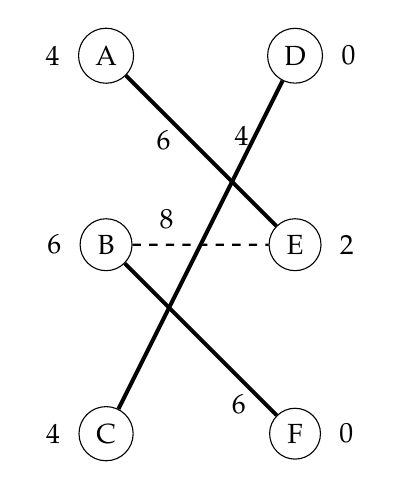
\begin{tikzpicture}[scale=.8,auto=left,every node/.style={circle,draw=black}]
			%left nodes
			\node [label=left:{4}] (m1) at (7,10) {A};
			\node [label=left:{6}] (m2) at (7,7) {B};
			\node [label=left:{4}] (m3) at (7,4) {C};

			%right nodes
			\node [label=right:{0}] (m4) at (10,10) {D};
			\node [label=right:{2}] (m5) at (10,7) {E};
			\node [label=right:{0}] (m6) at (10,4) {F};
			
			%edges
			\draw[line width=0.5mm] (m1) -- node[near start, draw=none, below] {6} ++ (m5);
			\draw[thick,dashed] (m2) -- node[near start, draw=none, above] {8} ++ (m5);
			\draw[line width=0.5mm] (m2) -- node[near end, draw=none, below] {6} ++ (m6);
			\draw[line width=0.5mm] (m3) -- node[near end, draw=none, above] {4} ++ (m4);
		\end{tikzpicture}
		\caption{Equality graph after augmenting.}
	\end{figure}
	This is a perfect matching on the equality graph, so this matching must be a maximum weight 
	matching on the graph. We can check that the values of the primal and dual solutions agree. 
	The sum of weights in the matching is $6+6+4 = 16$, and the sum of the values of our 
	dual variables is $4+6+4+2 = 16$.

	Note that if we want to just find a maximum cardinality matching on a bipartite graph, 
	we can just give all edges weight one and run this algorithm.

	This algorithm was one of the first primal-dual algorithms developed, and it anticipated many 
	later variations on the same theme. It displays the surprising connection between combinatorial 
	optimization and linear programming, which we explore in the next section.
\end{section}


\chapter{General primal-dual method and auction algorithms}

	In this chapter we will take a step back and look at primal-dual algorithms in more generality. 
	The goal will be to describe a method of solving a set of primal-dual algorithms for 
	\emph{network design problems}. Again, we will be restricting our attention to bipartite 
	graphs. In network design problems we are given a graph $G = (U,V,E)$ 
	and a cost $c_{uv}$ for each edge $(u,v)\in E$, and the goal is to find a minimum/maximum-cost 
	subset 
	$E\' \subset E$ that satisfies some criteria. Our maximum-cost matching problem is an example
	of this. There are other common examples that we will explore later on, but for now it suffices 
	to just think of these problems as choosing subsets of our graph according to some 
	stipulations. Throughout, we will be looking at undirected graphs.
\begin{section}{The Classical Primal-Dual Method}
	We begin by looking at what's known as the ``classical'' primal-dual method, which is concerned 
	with linear programs for polynomial-time solvable optimization problems. This will allow us 
	to build up a framework for a more general primal-dual method that we can use for approximation 
	algorithms - i.e. for problems that are known to be $NP$-hard. **(Not sure if this is within the 
	scope of the thesis -- discuss with Jim)\\
	Let's consider the linear program
	\begin{alignat}{2}
		& \text{minimize} & \mathbf{c}^{T}\mathbf{x} \\
		& \text{subject to } & A\mathbf{x} & \geq \mathbf{b} \\
		&& \mathbf{x} & \geq 0
	\end{alignat}
	and its dual
	\begin{alignat}{2}
		& \text{maximize} & \mathbf{b}^{T}\mathbf{y} \\
		& \text{subject to } & A^{T}\mathbf{y} & \leq \mathbf{c} \\
		&& \mathbf{y} & \geq 0.
	\end{alignat}
	We first define a concept that we will use throughout the rest of this thesis. 
	\begin{definition}{(Complementary slackness)}
		Given two linear programs in the form above, the \emph{primal complementary slackness 
		conditions} are the conditions which, given primal solution $\mathbf{x}$, 
		are necessary for a dual solution $\mathbf{y}$:
		\[
			x_j > 0 \implies A^{j}\mathbf{y} = c_j,
		\]
		where $A^{j}$ is the $j$th column of $A$. Similarly, the \emph{dual complementary 
		slackness conditions} are the conditions which, given dual solution $\mathbf{y}$, are 
		necessary for a primal solution $\mathbf{x}$:
		\[
			y_i > 0 \implies A_i\mathbf{x} = b_i,
		\]
		where $A_i$ is the $i$th row of $A$. Together, these conditions give us necessary and 
		sufficient conditions for solving the primal-dual system, which we will prove. The 
		(maximization) primal slackness variables are given by 
		$\mathbf{s} = \mathbf{b} - A\mathbf{x}$. The dual slackness variables are given by 
		$\mathbf{t} = A^{T}\mathbf{y} - \mathbf{c}$.
	\end{definition}
	\begin{theorem}{}
		[CITE THIS THEOREM]
		Let $\mathbf{x}$ be a primal feasible solution, and $\mathbf{y}$ a dual feasible 
		solution. Let $\mathbf{s}$ and $\mathbf{t}$ be the corresponding slackness variables. 
		Then $\mathbf{x}$ and $\mathbf{y}$ are optimal solutions if and only if the following 
		two conditions hold:
		\begin{align}
			x_jt_j &= 0 \quad \forall j \\
			y_is_i &= 0 \quad \forall i.
		\end{align}
	\end{theorem}
	\begin{proof}
		Let $u_i = y_is_i$ and $v_j = x_jt_j$, and $\mathbf{u} = \sum_i u_i$, 
		$\mathbf{v} = \sum_j v_j$. Then $\mathbf{u} = 0$ and $\mathbf{v} = 0$ if and only if 
		(7) and (8) hold. Also, 
		\begin{align*}
			\mathbf{u} + \mathbf{v} &= \sum y_is_i + \sum x_jt_j \\
						&= \sum y_i(b_i - A_ix_i) + \sum x_j (A^{T}_jy_j-c_j)\\
						&= \sum b_iy_i - \sum c_jx_j,
		\end{align*}
		so we get that $c^{T}\mathbf{x} = b^{T}\mathbf{y}$ if and only if $u + v = 0$, which 
		proves the statement.	
	\end{proof}
	The general ``tug-of-war'' between the primal and dual suggests an economic interpretation 
	of slackness conditions. We can think of our primal (maximization) problem as concerned with 
	profit given some constraints on resources, i.e. a resource allocation problem. The dual can 
	be interpreted as a valuation of the resources -- it tells us the availability of a resource, 
	and its price. So if we have optimal $\mathbf{x}$ and $\mathbf{y}$, we can interpret 
	slackness as follows: if there is slack in a constrained primal resource $i$ ($s_u > 0$), 
	then additional units of that resource must have no value ($y_u = 0$); if there is slack 
	in the dual price constraint ($t_v > 0$) there must be a shortage of that resource ($x_v = 0$).\\
	We now give an example of complementary slackness in action. Let's look back to our maximum 
	weight matching problem.Recall the primal linear program for maximum-weight matching:
	%Maximum matching ILP%
	\begin{alignat}{3}
		& \text{maximize } & \sum_{u,v} c_{uv} x_{uv}& \\
		& \text{subject to } \quad & \sum_{v} x_{uv} & \leq 1, & \quad \forall u\in U&, \\
				     &\quad & \sum_{u} x_{uv} & \leq 1, & \quad \forall v\in V &, \\
				&& x_{uv} & \geq 0.
	\end{alignat}
	and its dual
	%Vertex cover ILP%
	\begin{alignat}{3}
		& \text{minimize } & \sum_u y_u + \sum_v y_v& \\
		& \text{subject to } \quad & y_u + y_v & \geq c_{uv} & \quad \forall 
					u\in U,\ v\in V &, \\
				    && y_u,y_v & \geq 0.
	\end{alignat}
	The format here is a little different, since our primal is a maximization problem and the dual 
	is a minimization, but it's easy enough to reverse the roles. It's easy to see our 
	corresponding primal complementary slackness conditions are
	\begin{equation}
		x_{uv} > 0 \implies y_u + y_v = c_{uv}.
	\end{equation}
	The dual complementary slackness conditions are
	\begin{align}
		y_u > 0 &\implies \sum_v x_{uv} = 1,\\
		y_v > 0 &\implies \sum_u x_{uv} = 1.
	\end{align}
	In general, the slackness conditions guide us in our algorithm -- they tells us how, given a 
	solution to one of the problems, we should augment the solution to the other. For example, the 
	algorithm we presented for maximum-weight matching/minimum vertex cover intializes with 
	a solution to both the primal and dual that satisfies conditions (8) and (10); the algorithm 
	then at each step works to decrease the number of conditions in (9) that are unsatisfied, while 
	maintaining satisfiability of (8) and (10). This method is not unique to the Hungarian 
	algorithm. In fact, the Hungarian algorithm paved the way for this general method, which we 
	describe presently.\\
	Looking back at the original linear programs at the beginning of this chapter, suppose we have 
	a dual feasible solution $\mathbf{y}$. We can then state the problem of finding a feasible 
	primal solution $\mathbf{x}$ that obeys our complementary slackness conditions as another 
	\emph{restricted} linear program. Define the sets $A = \{j\ |\ A^{j}\mathbf{y} = c_j\}$ and 
	$B = \{i\ |\ y_i = 0\}$. So $A$ tells us which dual constraints (5) are tight, 
	given the solution $\mathbf{y}$, and $B$ tells us which $y_i$ are 0. What we want to do is 
	give a linear program to find a solution $\mathbf{x}$ that minimizes the 
	``violation'' of the complementary slackness conditions and the primal constraints, and to do 
	so we will index our variables by these sets. We will 
	have slack variables $s_i$ which will describe the difference between $A_i\mathbf{x}$ and $b_i$ 
	for $i\notin A$. We do this because we want to look at all $y_i > 0$ where the we do not 
	have that $A_i\mathbf{x} = b_i$. So part of our objective function will be to minimize the 
	sum of these $s_i$. We also want to minimize the sum over variables $x_j$ where $j\notin A$. 
	This is because we want to see if there are any $x_j$ such that $A^{j}\mathbf{y} \neq c_j$. 
	So we give the following restricted primal linear program:
	\begin{alignat}{3}
		& \text{minimize } & \sum_{i\notin B} s_i + \sum_{j\notin A} x_j & \\
		& \text{subject to } & A_i\mathbf{x} & \geq b_i & \quad i\in B &, \\
				     && A_i\mathbf{x} - b_i & = s_i & \quad i\notin B &, \\
				     && \mathbf{x} & \geq 0, \\
				     && \mathbf{s} & \geq 0.
	\end{alignat}
	Observe that if this restricted primal has a feasible solution $(\mathbf{x},\mathbf{s})$ such 
	that the objective function is 0, then $\mathbf{x}$ is a feasible primal solution that 
	satisfies the complementary slackness conditions for the dual solution $\mathbf{y}$. This 
	means that $\mathbf{x}$ and $\mathbf{y}$ are optimal primal and dual solutions. If, however, 
	the optimal solution to this restricted primal has value greater than 0, more work is required. 
	We can consider the dual of the restricted primal:
	\begin{alignat}{3}
		& \text{maximize } & \mathbf{b}^{T}\mathbf{w} & \\
		& \text{subject to } & A^{j}\mathbf{w} & \leq 0 & \quad j\in A &, \\
				     && A^{j}\mathbf{w} & \leq 1 & \quad j\notin A &, \\
				     && w_i\' & \geq -1 & \quad i\notin B &, \\
				     && w_i\' & \geq 0 & \quad i\in B &.
	\end{alignat}
	What we want here is to improve our dual solution. By assumption, the optimal solution to this 
	linear program's primal is greater than 0, so we know that this dual has a solution 
	$\mathbf{w}$ such that $\mathbf{b}^{T}\mathbf{w} > 0$. What we want is the existence of 
	some $\epsilon > 0$ such that $\mathbf{y}^{'} = \mathbf{y} + \epsilon \mathbf{w}$ is a 
	feasible dual solution. In particular, a solution of this form will be an improvement on our 
	original solution $\mathbf{y}$. We can calculate bounds on $\epsilon$ as follows. The two 
	conditions we must satisfy in order to maintain dual feasibility are that $y^{'} \geq 0$ and 
	$A^{T}y^{'} \leq c$. This means that we need 
	\begin{align}
		y_i + \epsilon w_i &\geq 0 \\
		A^{T}_j y + A^T_j \epsilon w & \leq c_j.
	\end{align}
	Let's consider the first one. When $w_i > 0$, we are fine; we need to be careful when 
	$w_i < 0$ since this could potentially violate the inequality. Solving in this way, we get 
	a first bound on $\epsilon$:
	\[
		\epsilon \leq \min_{i\in B: w_i < 0} (-y_i/w_i).
	\]
	Now let's address the second inequality. When $A^{T}_jw \leq 0$, we are defintely okay. We 
	need to be careful about violating the constraint when $A^{T}w > 0$. Thus, we can calculate a 
	second bound on $\epsilon$:
	\[
		\epsilon \leq \min_{j\in A: A^{T}_jw > 0} \frac{c_j-A^{T}_jy}{A^{T}_j w}.
	\]
	If we choose the lower of these two $\epsilon$ values, we obtain a new feasible dual solution 
	that has greater objective value. We can then work by reiterating the procedure, with the hope 
	that we find an optimal primal solution.\\
	It's not immediately clear why reducing our original linear programs to a series of linear 
	programs is heplful. However,  note that the vector $\mathbf{c}$ has totally disappeared in 
	the restricted primal and its dual. Recall that in the original linear program, $\mathbf{c}$ 
	gave us the edge-costs on our graph. So this method reworks our original weighted problem 
	into unweighted parts, which are easier to solve. Oftentimes, it is the case that 
	we can interpret these unweighted problems as purely combinatorial problems, which means that 
	instead of actually solving the problem with linear programming, we can solve it by 
	combinatorial 
	methods. Using a combinatorial algorithm to find a solution $\mathbf{x}$ that obeys the 
	complementary slackness conditions, or to find an improved dual solution $\mathbf{y}$, is 
	oftentimes more efficient.
\end{section}
	
\begin{section}{Primal-dual method for weighted matchings}
	Let us now look at an example of this method. We will look at a weighted matching problem, as 
	in the previous chapter, but this time we will look at \emph{minimizing} the cost of the 
	matching, instead of maximizing. We do this mainly because it illustrates something important 
	about the underlying structure of these matching problems. It will be easy to see how the 
	same method can be used for the case in which we want a maximimum matching. So the primal 
	linear program for a minimum weight perfect matching on a bipartite graph is given as follows. 
	\begin{alignat}{3}
		& \text{minimize } & \sum_{u,v} c_{uv} x_{uv}& \\
		& \text{subject to } \quad & \sum_{v} x_{uv} & \geq 1, & \quad \forall u\in U&, \\
				     &\quad & \sum_{u} x_{uv} & \geq 1, & \quad \forall v\in V &, \\
				&& x_{uv} & \geq 0.
	\end{alignat}
	Its dual is
	\begin{alignat}{3}
		& \text{maximize } & \sum_{u}y_u + \sum_{v}y_v & \\
		& \text{subject to } \quad & y_u + y_v & \leq c_{uv} & \quad \forall 
					u\in U,\ v\in V &, \\
				    && y_u,y_v & \geq 0.
	\end{alignat}
	We need to start with a dual feasible solution, and try to find a primal solution that 
	minimizes the violation of the constraints and slackness conditions. We can start with the 
	trivial dual solution of $y_u,y_v = 0$ for all $u,v$. Let's now think about our primal 
	complementary slackness. The set $A$ is given by $\{(u,v)\in E\ :\ y_u + y_v = c_{uv}\}$. 
	We know that these are the edges we want to include in our matching, and since we know our 
	linear program has integer solutions at extreme points of the polyhedron, let's specify that 
	$x_{uv} = 0$ for $(u,v)\notin a$. Now, our other slackness variables $s_u,s_v$ look like 
	\begin{align*}
		\sum_{v:(u,v)\in E} x_{uv} - s_u &= 1 \\
		\sum_{u:(u,v)\in E} x_{uv} - s_v &= 1.
	\end{align*}
	So we want to minimize over the sum of $s_u$ and $s_v$. Note that at this point, our set $B$ 
	consists of all vertices. So our restricted primal linear program is
	\begin{alignat}{3}
		& \text{minimize } & \sum_{u\in U} s_u + \sum_{v\in v} s_v & \\
		& \text{subject to } & \sum_v x_{uv} - s_u & = 1 & \quad \forall u &, \\
				     && \sum_u x_{uv} - s_v & = 1 & \quad \forall v &, \\
				     && x_{uv} & = 0 & \quad (u,v)\notin A, \\
				     && x_{uv} & \geq 0 & \quad (u,v)\in A, \\
				     && \mathbf{s} & \geq 0.
	\end{alignat}
	Let's first observe that all components of this restricted primal take on values 0 or 1, as 
	in the original primal. Moreover, note that we have turned a weighted problem into an 
	unweighted combinatorial problem. We've specified that we are not including any edge 
	$(u,v)\notin A$ in our matching, and we are trying to include as many $(u,v)\in A$ as possible 
	in our matching by minimizing the slackness variables. Note that the graph $G^{'} = (U,V,J)$ 
	is exactly the equality subgraph as defined in the previous chapter! In our Hungarian algorithm 
	we repeatedly sought to find maximum cardinality matchings within this subgraph, which is 
	exactly what this restricted primal is having us do. This tells us that the problems of maximum 
	weight matching and minimum weight matching only differ in the labeling we are specifying. The 
	underlying procedure for solving both of the problems is essentially the same. So if we find a 
	perfect matching in $G^{'}$, we will have found an $\mathbf{x}$ that obeys the complementary 
	slackness conditions, i.e. $\sum_u s_u + \sum_v s_v = 0$. Moreover, this implies that the 
	dual solution $\sum_u y_u + \sum_v y_v$ must be optimal as well.\\
	Now, if the solution $\sum_u s_u + \sum_v s_v > 0$, we do not have an optimal $\mathbf{x}$, 
	so we need to adjust our dual. We look at this now, in the dual linear program of the 
	restricted primal.
	\begin{alignat}{3}
		& \text{maximize } & \sum_{u\in U} w_u + \sum_{v\in V} w_v & \\
		& \text{subject to } & w_u + w_v & \leq 0 & \quad \forall (u,v)\in A &, \\
				     && w_u + w_v & \leq 1 & \quad \forall (u,v)\notin A &, \\
				     && w_u,w_v & \geq -1 & \quad u,v\notin B, \\
				     && w_u,w_v & \geq 0 & \quad u,v\in B, \\
				     && \mathbf{w} & \geq 0.
	\end{alignat}
	We now want to find an $\epsilon$ such that the solution $z = \sum_u y_u + \sum_v y_v + 
	\epsilon (\sum_u w_u + \sum_v w_v)$ is (1) feasible and (2) an improvement of the dual 
	objective. First of all, we know that since the restricted primal has solution $\geq 0$, 
	the solution to this dual will also be $\geq 0$. So we just need to worry about the condition 
	\[
		y_u + y_v + \epsilon (w_u + w_v) \leq c_{uv}.
	\]
	So we get that we at least need that $\epsilon \leq \min_{(u,v)\notin A: w_u + w_v > 0}
	\frac{c_{uv} - y_u - y_v}{w_u + w_v}$. We can refine this by noting that since 
	$0 < w_u + w_v \leq 1$ for $(u,v)\notin A$, we have $\epsilon = \min_{(u,v)\notin A} 
	(c_{uv} - y_u - y_v)$. Note that the negative of this is exactly the quantity we modify our 
	labeling by in the Hungarian algorithm in the previous chapter. Thus we've found an 
	$\epsilon$ that maintains dual feasibility, and increases the objectie function. We can use 
	this solution and revisit the restricted primal in order to look for an improved feasible 
	primal solution.
\end{section}

\begin{section}{Auction algorithms}
	We now look at a cool application of weighted bipartite matching. Let's imagine our assignment 
	problem is an auction. We will motivate this through an economic lens. Suppose that a good $g$ 
	has a price $p_g$, and a buyer $b$ must pay $p_g$ to receive this item. Suppose that the 
	amount $b$ is willing to pay for $g$, or $b$'s valuation of $b$, is $c_{bg}$. Then the net value 
	of this item to $b$ is $c_{bg} - p_g$. Assuming that each bidder $b$ is a rational agent acting 
	in their own best interest, each $b$ would want to be assigned a good $g$ that maximizes their 
	net value, i.e. for all $b$ with good $g$, we have that 
	\[
		c_{bg} - p_g = \max_g \{c_{bg} - p_g \}.
	\]
	This would give us an economic system in equilibrium; no bidder would have an incentive to 
	seek/trade for a different good.
	The reason this is of interest to us is that an equilibrium assignment maximizes total 
	profit (i.e. it solves the primal linear program for maximum weight matchings), while the 
	corresponding set of prices solves the associated dual problem.\\
	Our goal is to maximize the total amount earned in the auction -- i.e. to 
	maximize $\sum_{(b,g)} c_{bg}$, under the constraint that no bidder gets more than one good, 
	and no good is purchased by more than one bidder. \\
	At a general step in our algorithm, we will want to consider a bidder $b$ that is currently 
	not the owner of any good, and find a good $g$ that maximizes $c_{bg} - p_g$. We will then need 
	to do to things: (1), replace the current owner of $g$ (put them back into the set of unassigned 
	bidders) with $b$; (2) bump the price of $g$ by some amount $\delta$. 
	Step (2) is tricky to figure out. Bertsekas [CITE] describes in detail the process of finding a 
	good $\delta$ and, more importantly, what values of $\delta$ to avoid. Here we leave out the 
	details of finding a decent $\delta$. We first present the algorithm with a given $\delta$, and 
	then analyze why it is a good choice.
	\singlespace
	\begin{codebox}
		\Procname{$\proc{Alg 1}$}
		\li For each $g\in G$, set $p_g \gets 0$ and $owner_g \gets null$.
		\li Queue $Q \gets B$.
		\li Set $\delta = 1/(|G| + 1)$.
		\li \While $Q\neq \emptyset$
			\Do
		\li		$b = Q.deque()$
		\li		Find $g\in G$ that maximizes $c_{bg} - p_{g}$
		\li		\If $c_{bg} - p_{g} \geq 0$
					\Then
		\li				$Q.enqueue(owner_g)$
		\li				$owner_g = b$
		\li				$p_g = p_g + \delta$
					\End
			\End
		\li \Return $(owner_g,g)$ for all $g$.
	\end{codebox}
	\doublespacing
	\begin{definition}{}
		We say that a bidder $b$ is $\delta$-happy if one of the following is true:
		\begin{enumerate}
			\item $b$ is the owner of some good $g$, and for all other goods $g\'$, we have 
				that $\delta + c_{bg} - p_g \geq c_{bg\'} - p_{g\'}$, i.e. our $b$ 
				has the good $g$ that maximizes the value of their contribution.
			\item for no good $g$ does it hold that $owner_g = b$ and for all goods $g$ 
				$w_{bg} \leq p_g$.
		\end{enumerate}
	\end{definition}
	What we will show is that the algorithm reaches an equilibrium in which all bidders are 
	``happy,'' as defined above. The loop invariant is that all bidders not in $Q$ are $\delta$-
	happy. This is clearly true at the beginning, as all bidders start in our queue. When a bidder 
	$b$ is dequeued, line $6$ in our loop chooses good $g$ that maximizes $w_{bg} - p_g$, which 
	means it chooses a good that makes $b$ $\delta$-happy, if such a good exists. We need to confirm 
	that this step does not hurt the invariant for any other bidder $b\'$. Well, an increase in 
	$p_g$ by $\delta$ for any $g$ not owned by $b\'$ does not violate the inequality $\delta + 
	w_{b\' g\'} - p_{g\'} \geq w_{b\' g} - p_g$. On the other hand, if $b\'$ did own $g$, this means 
	that $b\'$ has been thrown back into $Q$, so $b\'$ no longer owns anything.
	\begin{lemma}{}
		If all bidders are $\delta$-happy then for every matching $M\'$ we have that 
		\[
			n\delta + \sum_{b = owner_g} w_{bg} \geq \sum_{(b,g)\in M\'} w_{bg},
		\]
		where $n$ is the number of bidders. 
	\end{lemma}
	First, note that this lemma implies the correctness of our algorithm. Since $n\delta < 1$ 
	and all of our weights are integral, proving this inequality will show that the matching we 
	output is a maximum matching.
	\begin{proof}
		Fix a bidder $b$, and let good $g$ be such that $b = owner_g$. Let $g\'$ be the good 
		assigned to $b$ in $M\'$. (Note: these could be \emph{null}, in which case we adopt the 
		convention of assigning their weights and prices to be zero.) Since $b$ is $\delta$-
		happy, we have that $\delta + w_{bg} - p_g \geq w_{bg} - p_g$. Now let's sum over all 
		$b$ to get 
		\[
			\sum_{b=owner_g} (\delta + w_{bg} - p_g) \geq \sum_{(b,g\')\in M\'} (w_{bg\'} - 
			p_g).
		\]
		We know that our algorithm gives us a matching, as does $M\'$, which means that each 
		good $g$ can only appear at most once on each side of this inequality. So if we subtract 
		$\sum_g p_g$ from each side, and rearrange a bit, we get 
		\[
			\sum_{b=owner_g} \delta + \sum_{b=owner_g} w_{bg} \geq \sum_{(b,g\')\in M\'} 
			(w_{bg\'}). 
		\]
		But $\sum_{b=owner_g} \delta \leq n\delta$, which gives us what we want.
	\end{proof}
	Let's think about how this algorithm relates to the corresponding primal and dual linear 
	programs. First, note that this algorithm maintains primal feasibility at all times, as each 
	good has at most one owner, and each bidder owns at most one good. However, at no point are we 
	maintaining dual feasibility. We can define the ``price'' on bidders $b$ as $p_b = 0$ for all 
	$b$. Furthermore, the prices on goods $p_g$ never exceed $\max_{b} \{w_{bg}\}$. We can think of 
	these $p_b$ and $p_g$ as the corresponding dual variables in the dual linear program. 
	Throughout the course of this algorithm, we never have that $p_b + p_g \geq w_{bg}$, which 
	means that we are violating our primal complementary slackness conditions. Note however that 
	we do maintain the dual complementary slackness conditions. 
	It is still useful to think about this algorithm in terms of the linear programs since, although 
	infeasible as a dual solution, our final price vector $\mathbf{p}$ is the pointwise minimum 
	such that all bidders are $\delta$-happy. So the algorithm is still performing a minimization 
	over $\sum_b p_b + \sum_g p_g = \sum_g p_g$, but relaxing the constraint that $p_b + p_g = 
	p_g \geq w_{bg}$.\\
\end{section}

	



\backmatter % backmatter makes the index and bibliography appear properly in the t.o.c...

% if you're using bibtex, the next line forces every entry in the bibtex file to be included
% in your bibliography, regardless of whether or not you've cited it in the thesis.
    %\nocite{*}

% Rename my bibliography to be called "Works Cited" and not "References" or ``Bibliography''
% \renewcommand{\bibname}{Works Cited}

%    \bibliographystyle{bsts/mla-good} % there are a variety of styles available; 
%  \bibliographystyle{plainnat}
% replace ``plainnat'' with the style of choice. You can refer to files in the bsts or APA 
% subfolder, e.g. 
% \bibliographystyle{APA/apa-good}  % or
% \bibliography{thesis} THIS LINE AND LINE ABOVE FOR REFERENCES
 % Comment the above two lines and uncomment the next line to use biblatex-chicago.
 %\printbibliography[heading=bibintoc]

% Finally, an index would go here... but it is also optional.
\end{document}
